\documentclass[11pt,a4paper]{article}

\usepackage[utf8]{inputenc}
\usepackage[T1]{fontenc}
\usepackage{lmodern}
\usepackage[margin=2.4cm]{geometry}
\usepackage{graphicx}
\usepackage{booktabs}
\usepackage{caption}
\usepackage{subcaption}
\usepackage{float}
\usepackage{amsmath}
\usepackage[hidelinks]{hyperref}

\graphicspath{{../results/}}
\captionsetup{font=small,labelfont=bf}
\setlength{\parskip}{0.4em}
\setlength{\parindent}{0pt}

\title{\textbf{COVID-19 CT Multi-class Segmentation:\\
U-Net vs.\ DeepLabV3+ with Optuna Hyperparameter Search}}
\author{Nick Kantiotis\\\small MSc Artificial Intelligence \& Visual Computing (AIVC)}
\date{\today}

\begin{document}
\maketitle

\begin{abstract}
\noindent
We address pixel-wise semantic segmentation of chest CT scans into four classes
---\,\emph{background}, \emph{left lung}, \emph{right lung} and \emph{infection}\,---
on the public COVID-19 CT Lung and Infection dataset (20 annotated volumes, Zenodo
3757476). Two encoder--decoder architectures, \textbf{U-Net} and \textbf{DeepLabV3+},
are trained on 2D axial slices with a combined Dice + Cross-Entropy loss, and tuned with
\textbf{Optuna} (5 trials each, maximising validation foreground Dice). On a held-out,
patient-level test split, \textbf{U-Net} attains a mean foreground Dice of \textbf{0.915}
(IoU 0.854) versus \textbf{0.858} (IoU 0.782) for DeepLabV3+. The gap is driven almost
entirely by the small, imbalanced \emph{infection} class (Dice 0.794 vs.\ 0.635), where
DeepLabV3+ under-segments lesions (sensitivity 0.50 vs.\ 0.77).
\end{abstract}

\tableofcontents
\bigskip

%==================================================================
\section{Introduction}
%==================================================================
The COVID-19 CT Lung and Infection Segmentation dataset~\cite{ma2020} contains
\textbf{20 labelled CT volumes} (NIfTI \texttt{.nii.gz}) from the Coronacases Initiative
and Radiopaedia, annotated by radiologists into left lung, right lung and infection.
The task is to segment each axial slice into these structures, supporting automated
assessment of COVID-19 lung involvement. We compare two widely used segmentation
networks under an identical training and tuning protocol to isolate the effect of
architecture, with particular attention to the clinically critical but hardest target:
the infection (lesion) class.

%==================================================================
\section{Dataset}
%==================================================================
The dataset provides 20 three-dimensional CT volumes with dense voxel labels over four
classes (Table~\ref{tab:classes}). Annotations are released under the
\textbf{CC BY-NC-SA} licence~\cite{ma2020}.

\begin{table}[H]
\centering
\caption{Label encoding of the four segmentation classes.}
\label{tab:classes}
\begin{tabular}{cl}
\toprule
Index & Class \\
\midrule
0 & background \\
1 & left lung \\
2 & right lung \\
3 & infection (lesion) \\
\bottomrule
\end{tabular}
\end{table}

\textbf{Patient-level split.} The 20 volumes are split deterministically (seed 42) into
\textbf{14 train / 3 validation / 3 test} patients. Crucially, slices from a single volume
never cross splits, preventing data leakage and keeping the evaluation honest despite the
small number of subjects.

%==================================================================
\section{Methodology}
%==================================================================
\textbf{2D slice segmentation.} Each 3D volume is sliced along the axial axis, producing
thousands of 2D samples from only 20 volumes. Background-only slices (fewer than 50
foreground pixels) are discarded.

\textbf{Preprocessing.} Each slice is clipped to the lung Hounsfield-Unit window
$[-1250, 250]$, min--max normalised to $[0,1]$, resized to $256\times256$, and replicated
to 3 channels to match ImageNet-pretrained encoders.

\textbf{Loss.} We optimise a sum of multiclass \textbf{Dice loss} and
\textbf{Cross-Entropy}, which together handle the strong class imbalance (the infection
class occupies a tiny fraction of pixels).

\textbf{Optimisation.} Adam optimiser with a \texttt{ReduceLROnPlateau} schedule
(monitoring validation Dice) and early stopping (patience 10 epochs). Data augmentation
(Albumentations: flips, shift/scale/rotate, brightness/contrast) is applied at a strength
selected per trial during tuning.

%==================================================================
\section{Models}
%==================================================================
Both architectures are built with \texttt{segmentation\_models\_pytorch}, take a
$3\times256\times256$ input and output 4-channel per-class logits.

\begin{itemize}
  \item \textbf{U-Net} --- symmetric encoder--decoder with skip connections that recover
        spatial detail lost in downsampling. ($\approx$14.3\,M parameters with a ResNet18
        encoder.)
  \item \textbf{DeepLabV3+} --- atrous spatial pyramid pooling (ASPP) for multi-scale
        context aggregation. ($\approx$12.3\,M parameters with a ResNet18 encoder.)
\end{itemize}

The encoder is a tunable hyperparameter
(\texttt{resnet18} / \texttt{resnet34} / \texttt{efficientnet-b0}), initialised with
ImageNet weights. Optuna selected \texttt{resnet18} as the best encoder for both models.

%==================================================================
\section{Hyperparameter Search (Optuna)}
%==================================================================
Hyperparameters are tuned with \textbf{Optuna}~\cite{optuna} using a TPE sampler
(seed 42) and a \texttt{MedianPruner} (5 warm-up steps) to terminate unpromising trials.
We run \textbf{5 trials per model}, each up to 50 epochs, maximising the validation mean
foreground Dice. The search space spans learning rate ($10^{-5}$--$10^{-2}$, log scale),
batch size $\{4,8,16\}$, encoder
$\{$\texttt{resnet18}, \texttt{resnet34}, \texttt{efficientnet-b0}$\}$ and augmentation
strength $\{$none, light, strong$\}$. The best configurations are reported in
Table~\ref{tab:best}.

\begin{table}[H]
\centering
\caption{Best hyperparameters per model (Optuna).}
\label{tab:best}
\begin{tabular}{lcccc}
\toprule
Model & lr & batch size & encoder & aug.\ strength \\
\midrule
U-Net      & $6.65\times10^{-4}$ & 16 & resnet18 & light \\
DeepLabV3+ & $1.33\times10^{-4}$ & 4  & resnet18 & none  \\
\bottomrule
\end{tabular}
\end{table}

\begin{figure}[H]
\centering
\begin{subfigure}{0.48\textwidth}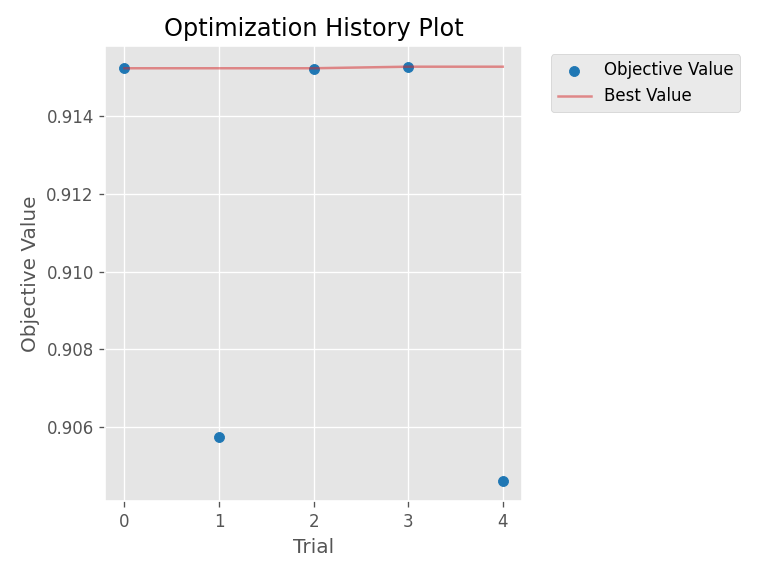
\includegraphics[width=\linewidth]{optuna_unet_history.png}
  \caption{Optimisation history}\end{subfigure}\hfill
\begin{subfigure}{0.48\textwidth}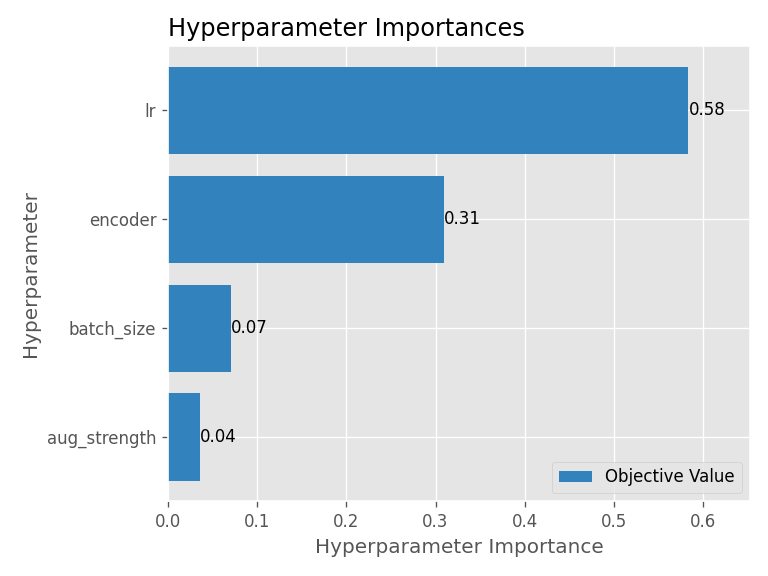
\includegraphics[width=\linewidth]{optuna_unet_importance.png}
  \caption{Parameter importance}\end{subfigure}
\\[0.4em]
\begin{subfigure}{0.48\textwidth}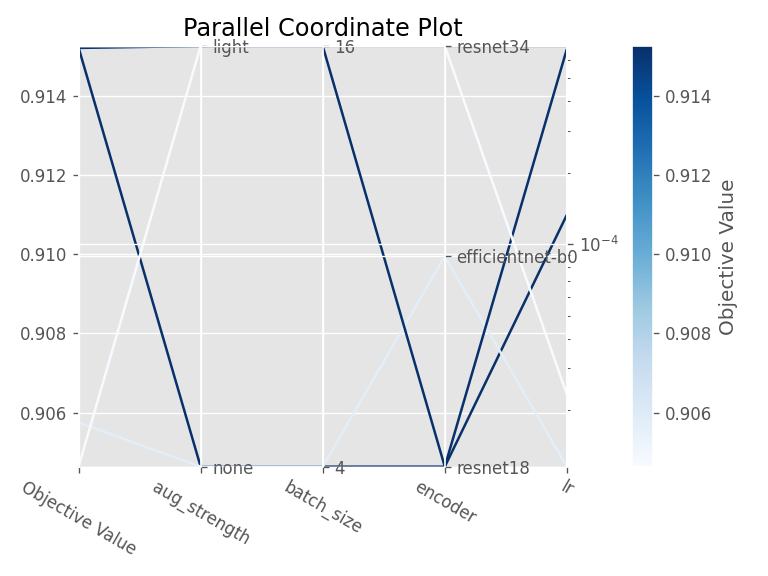
\includegraphics[width=\linewidth]{optuna_unet_parallel.png}
  \caption{Parallel coordinate}\end{subfigure}\hfill
\begin{subfigure}{0.48\textwidth}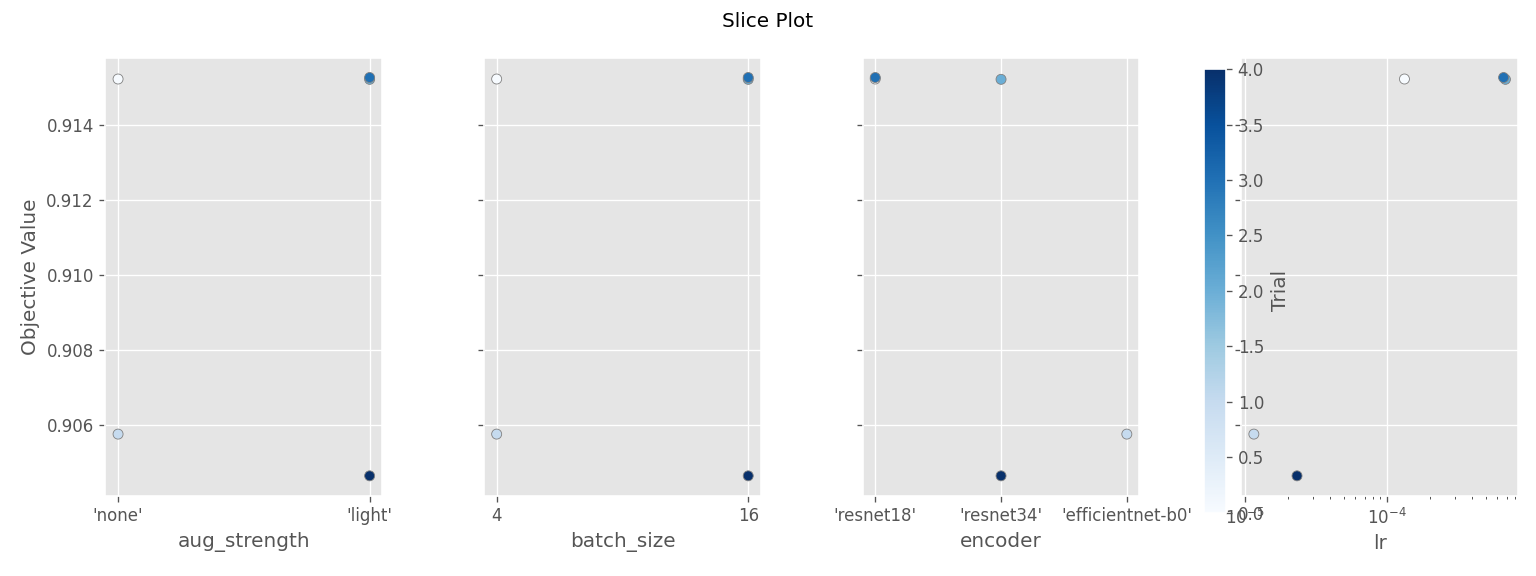
\includegraphics[width=\linewidth]{optuna_unet_slice.png}
  \caption{Slice plot}\end{subfigure}
\caption{Optuna study visualisations for \textbf{U-Net}.}
\label{fig:optuna-unet}
\end{figure}

\begin{figure}[H]
\centering
\begin{subfigure}{0.48\textwidth}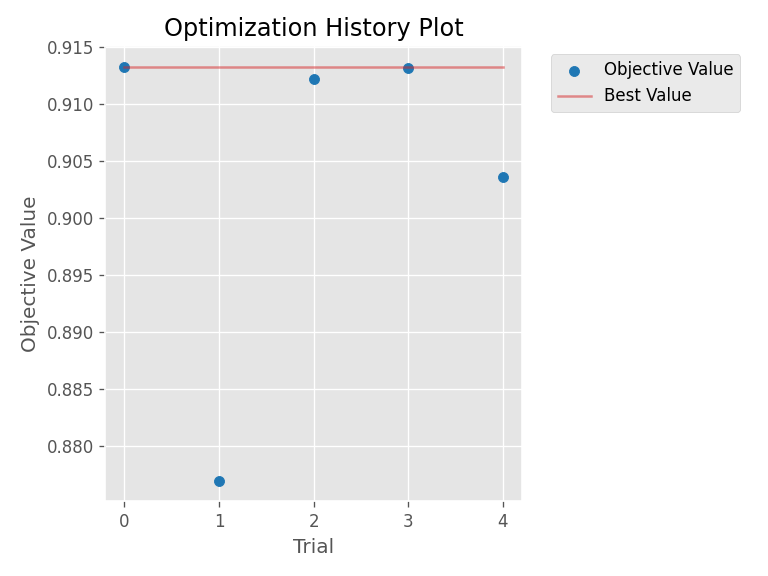
\includegraphics[width=\linewidth]{optuna_deeplabv3plus_history.png}
  \caption{Optimisation history}\end{subfigure}\hfill
\begin{subfigure}{0.48\textwidth}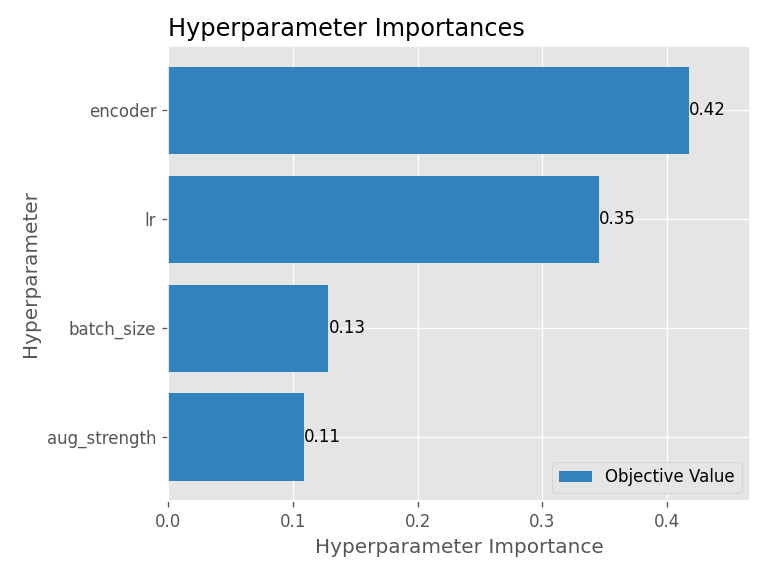
\includegraphics[width=\linewidth]{optuna_deeplabv3plus_importance.png}
  \caption{Parameter importance}\end{subfigure}
\\[0.4em]
\begin{subfigure}{0.48\textwidth}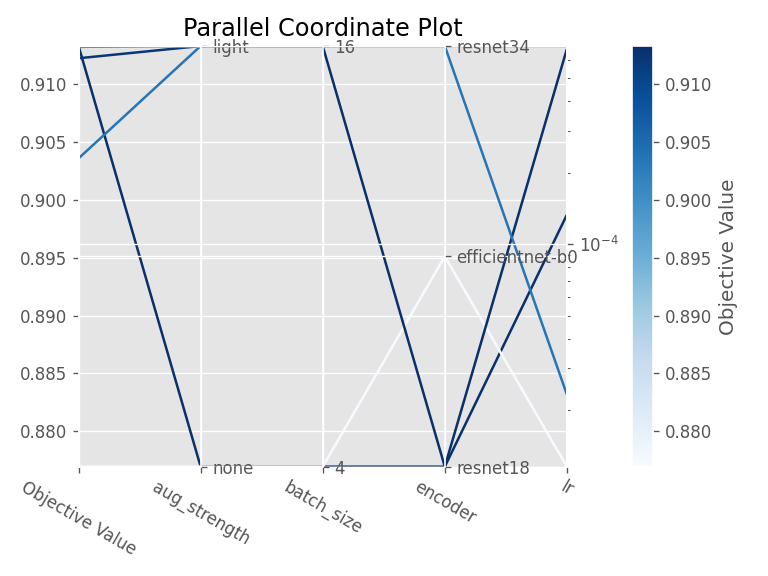
\includegraphics[width=\linewidth]{optuna_deeplabv3plus_parallel.png}
  \caption{Parallel coordinate}\end{subfigure}\hfill
\begin{subfigure}{0.48\textwidth}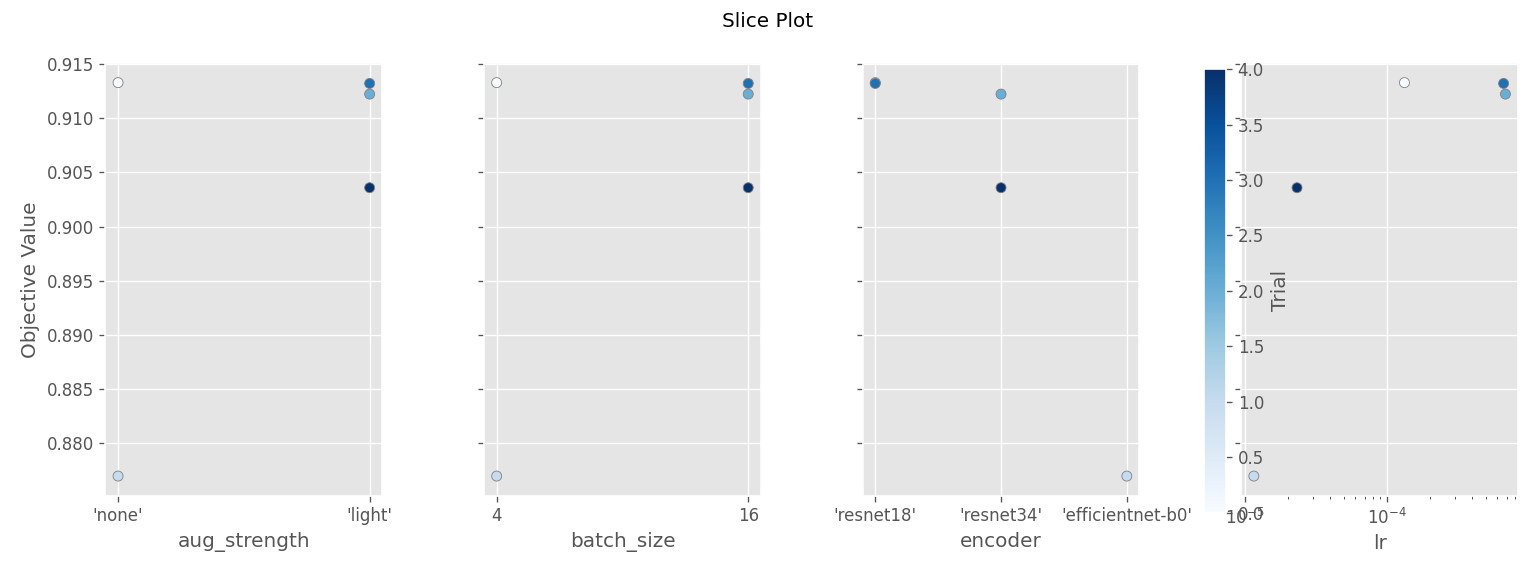
\includegraphics[width=\linewidth]{optuna_deeplabv3plus_slice.png}
  \caption{Slice plot}\end{subfigure}
\caption{Optuna study visualisations for \textbf{DeepLabV3+}.}
\label{fig:optuna-deeplab}
\end{figure}

%==================================================================
\section{Results}
%==================================================================
All metrics are computed on the held-out \textbf{test split} (3 patients, unseen during
training and tuning).

\begin{table}[H]
\centering
\caption{Test-set comparison. Best per column in \textbf{bold}.}
\label{tab:compare}
\begin{tabular}{lcccccc}
\toprule
Model & Dice left & Dice right & Dice infection & mean FG Dice & mean FG IoU & Params (M) \\
\midrule
\textbf{U-Net} & \textbf{0.980} & \textbf{0.971} & \textbf{0.794} & \textbf{0.915} & \textbf{0.854} & 14.3 \\
DeepLabV3+     & 0.978 & 0.960 & 0.635 & 0.858 & 0.782 & 12.3 \\
\bottomrule
\end{tabular}
\end{table}

U-Net wins overall, and the gap is driven almost entirely by the \emph{infection} class
(0.794 vs.\ 0.635 Dice) --- the hardest, smallest and most imbalanced structure. Per-class
metrics are detailed in Tables~\ref{tab:unet} and~\ref{tab:deeplab}.

\begin{table}[H]
\centering
\caption{U-Net per-class metrics.}
\label{tab:unet}
\begin{tabular}{lcccc}
\toprule
Class & Dice & IoU & Sensitivity & Specificity \\
\midrule
background & 0.998 & 0.996 & 0.998 & 0.986 \\
left\_lung & 0.980 & 0.960 & 0.976 & 0.999 \\
right\_lung & 0.971 & 0.944 & 0.982 & 0.998 \\
infection & 0.794 & 0.659 & 0.770 & 0.999 \\
\bottomrule
\end{tabular}
\end{table}

\begin{table}[H]
\centering
\caption{DeepLabV3+ per-class metrics.}
\label{tab:deeplab}
\begin{tabular}{lcccc}
\toprule
Class & Dice & IoU & Sensitivity & Specificity \\
\midrule
background & 0.998 & 0.995 & 0.998 & 0.979 \\
left\_lung & 0.978 & 0.957 & 0.981 & 0.999 \\
right\_lung & 0.960 & 0.923 & 0.978 & 0.997 \\
infection & 0.635 & 0.465 & 0.500 & 1.000 \\
\bottomrule
\end{tabular}
\end{table}

DeepLabV3+ reaches an infection \textbf{sensitivity of only 0.50} (vs.\ U-Net's 0.77) while
its specificity stays at 1.0 --- i.e.\ it under-segments the small lesions, missing half of
the infection pixels.

\subsection{Training curves (best trial)}
\begin{figure}[H]
\centering
\begin{subfigure}{0.49\textwidth}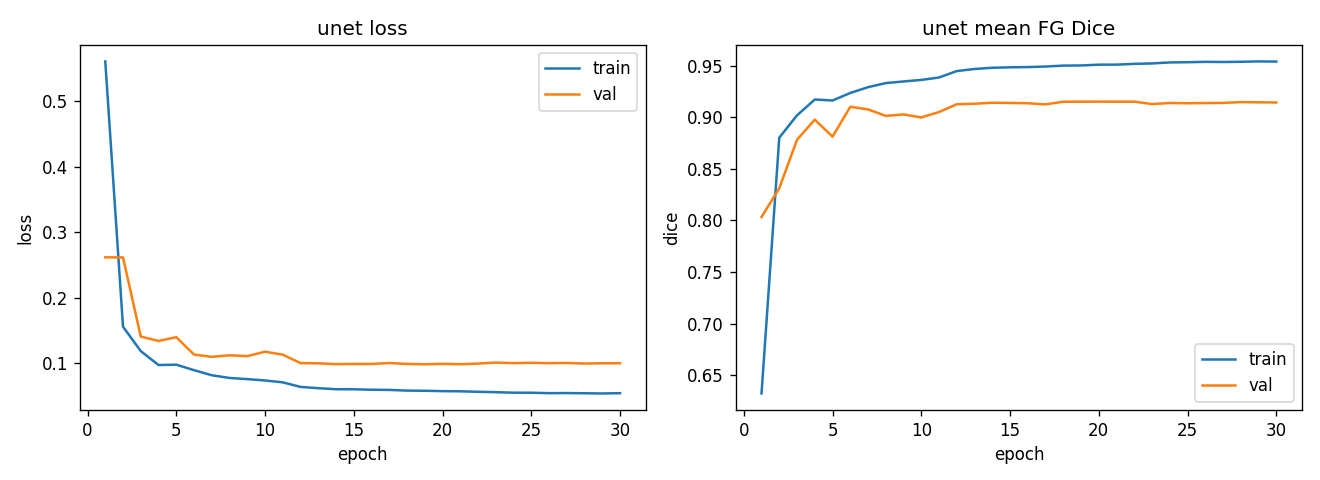
\includegraphics[width=\linewidth]{unet_curves.png}
  \caption{U-Net}\end{subfigure}\hfill
\begin{subfigure}{0.49\textwidth}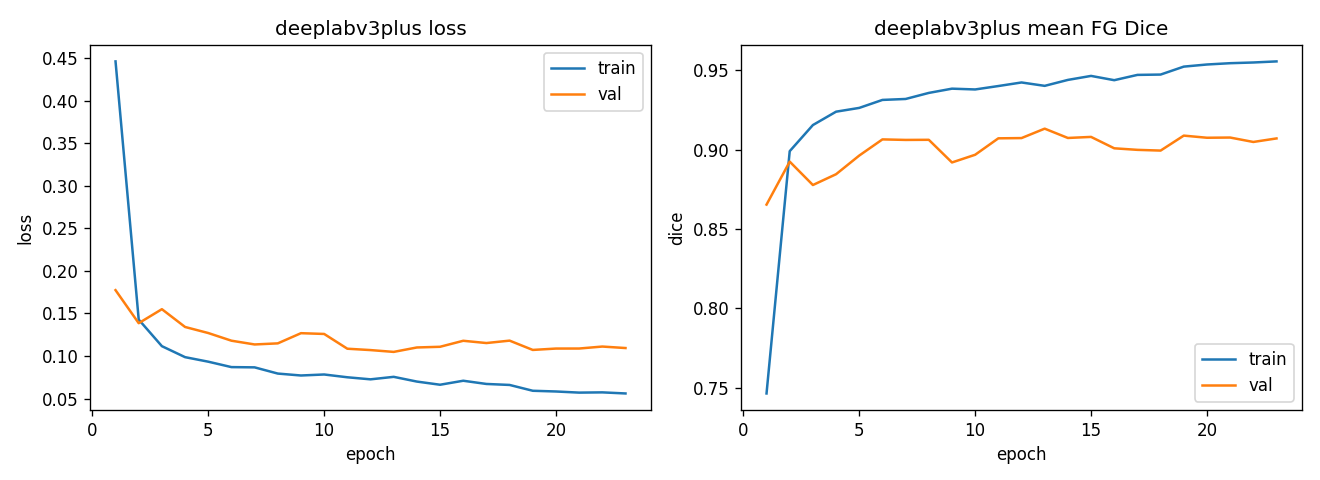
\includegraphics[width=\linewidth]{deeplabv3plus_curves.png}
  \caption{DeepLabV3+}\end{subfigure}
\caption{Loss and mean foreground Dice vs.\ epoch for the best trial of each model.}
\label{fig:curves}
\end{figure}

\subsection{Confusion matrices}
\begin{figure}[H]
\centering
\begin{subfigure}{0.49\textwidth}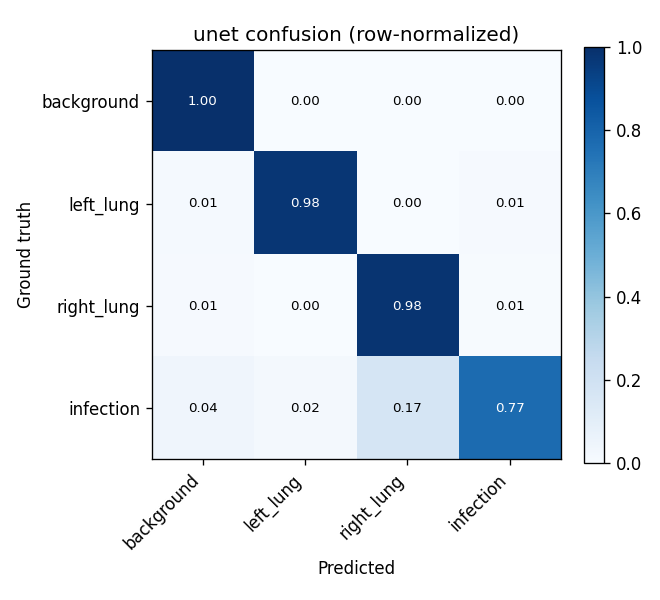
\includegraphics[width=\linewidth]{unet_confusion.png}
  \caption{U-Net}\end{subfigure}\hfill
\begin{subfigure}{0.49\textwidth}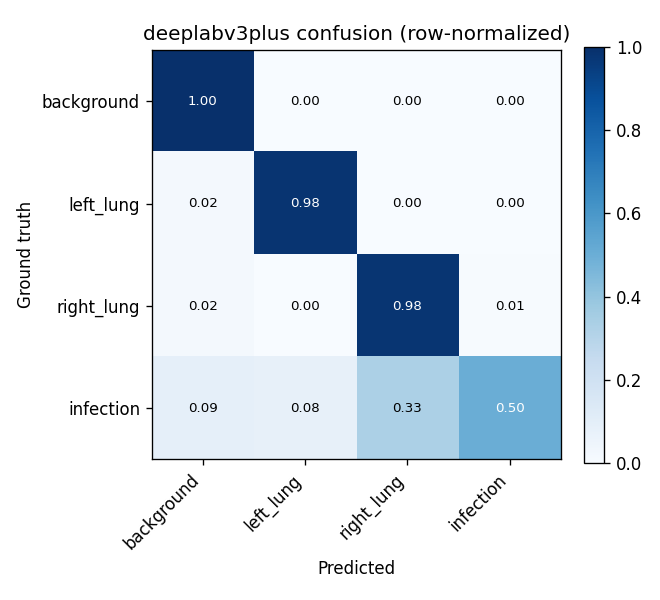
\includegraphics[width=\linewidth]{deeplabv3plus_confusion.png}
  \caption{DeepLabV3+}\end{subfigure}
\caption{Pixel-level, row-normalised confusion matrices over the four classes.}
\label{fig:confusion}
\end{figure}

\subsection{Qualitative overlays}
\begin{figure}[H]
\centering
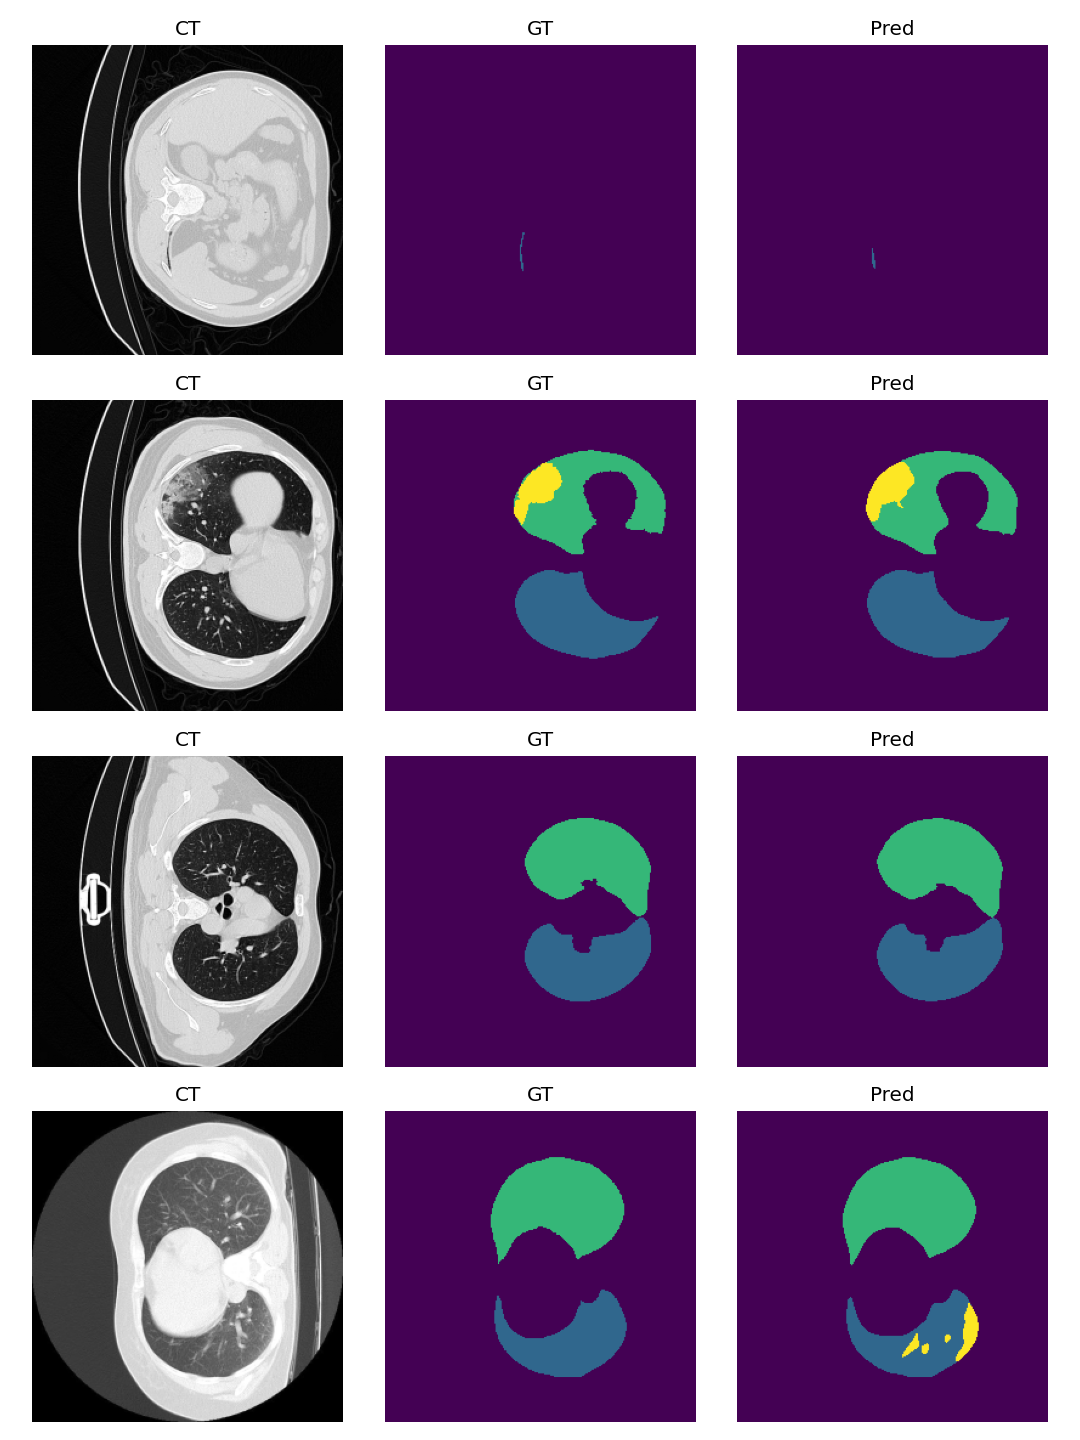
\includegraphics[width=0.92\textwidth]{unet_overlays.png}
\caption{U-Net qualitative results on test slices: CT / ground truth / prediction.}
\label{fig:unet-overlays}
\end{figure}

\begin{figure}[H]
\centering
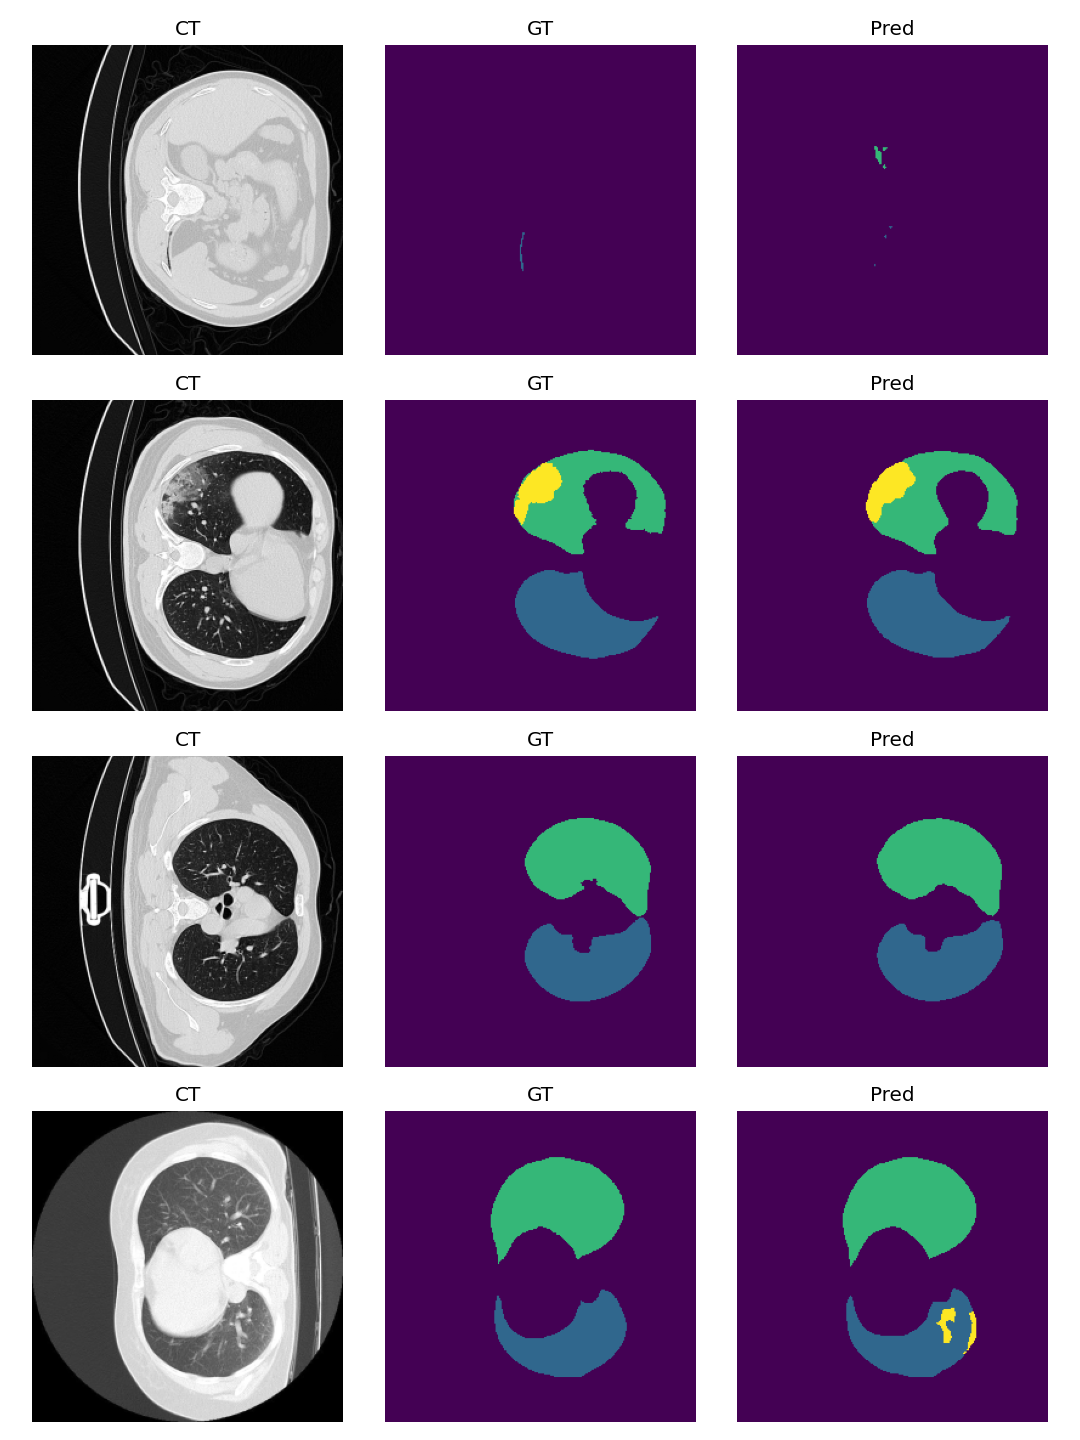
\includegraphics[width=0.92\textwidth]{deeplabv3plus_overlays.png}
\caption{DeepLabV3+ qualitative results on test slices: CT / ground truth / prediction.}
\label{fig:deeplab-overlays}
\end{figure}

\subsection{Per-trial training curves}
\begin{figure}[H]
\centering
\begin{subfigure}{0.32\textwidth}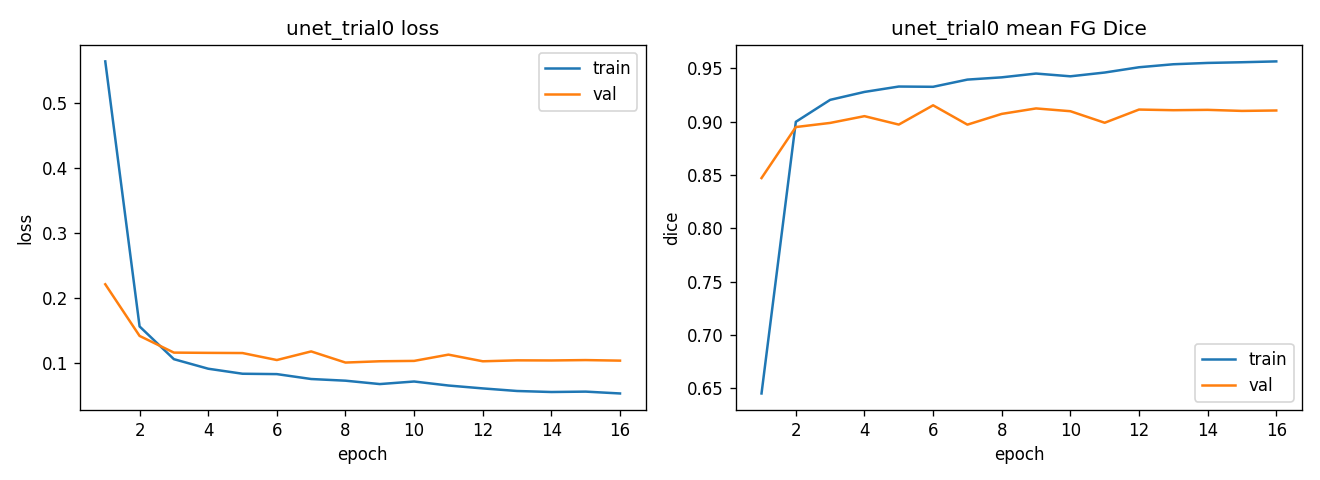
\includegraphics[width=\linewidth]{unet_trial0_curves.png}\caption{Trial 0}\end{subfigure}\hfill
\begin{subfigure}{0.32\textwidth}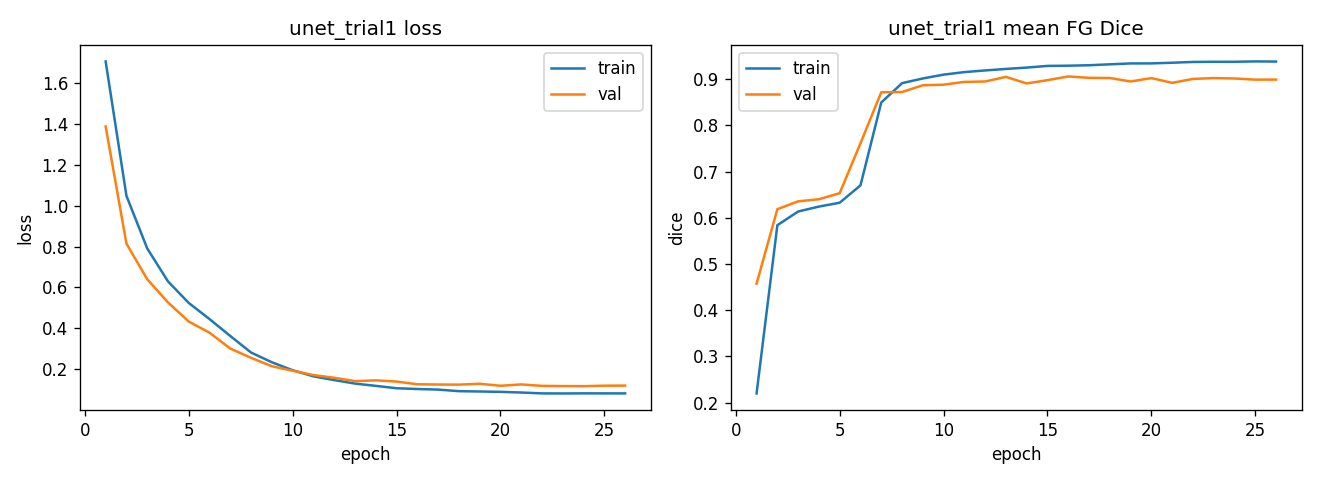
\includegraphics[width=\linewidth]{unet_trial1_curves.png}\caption{Trial 1}\end{subfigure}\hfill
\begin{subfigure}{0.32\textwidth}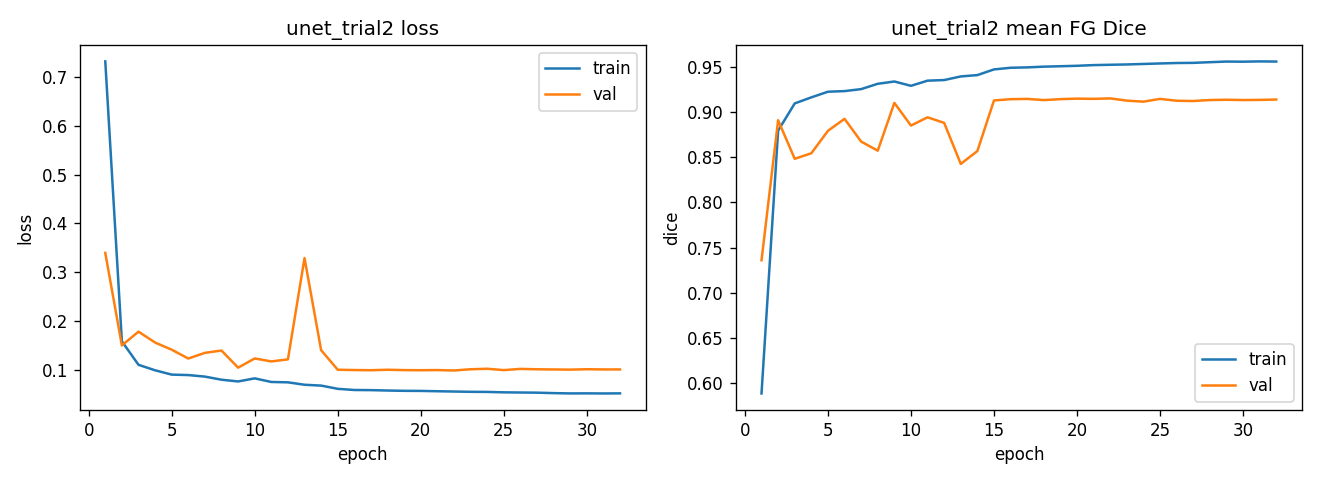
\includegraphics[width=\linewidth]{unet_trial2_curves.png}\caption{Trial 2}\end{subfigure}
\\[0.4em]
\begin{subfigure}{0.32\textwidth}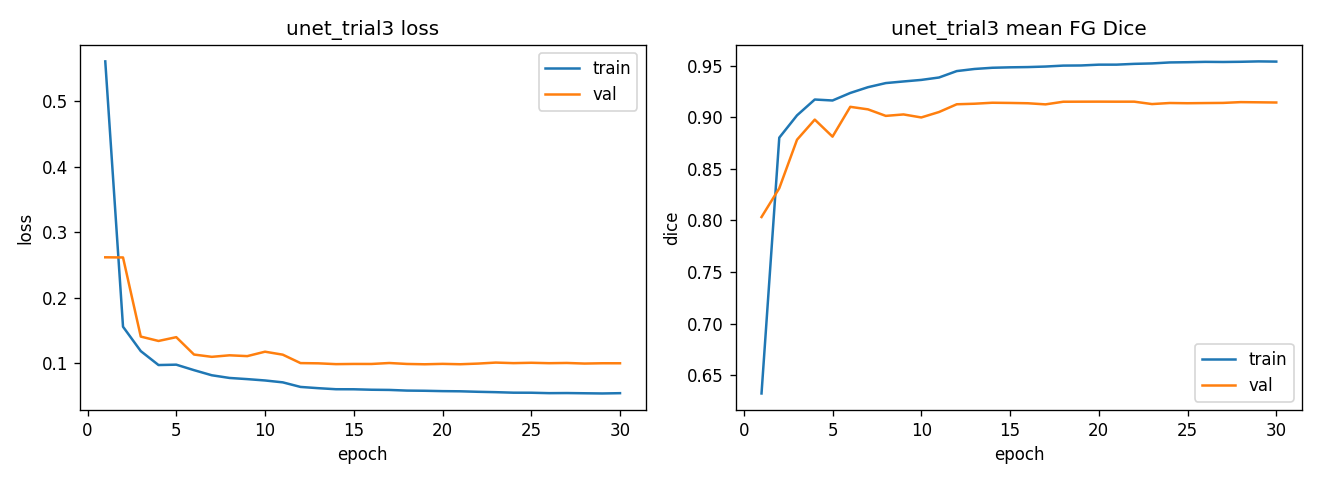
\includegraphics[width=\linewidth]{unet_trial3_curves.png}\caption{Trial 3 (best)}\end{subfigure}\hfill
\begin{subfigure}{0.32\textwidth}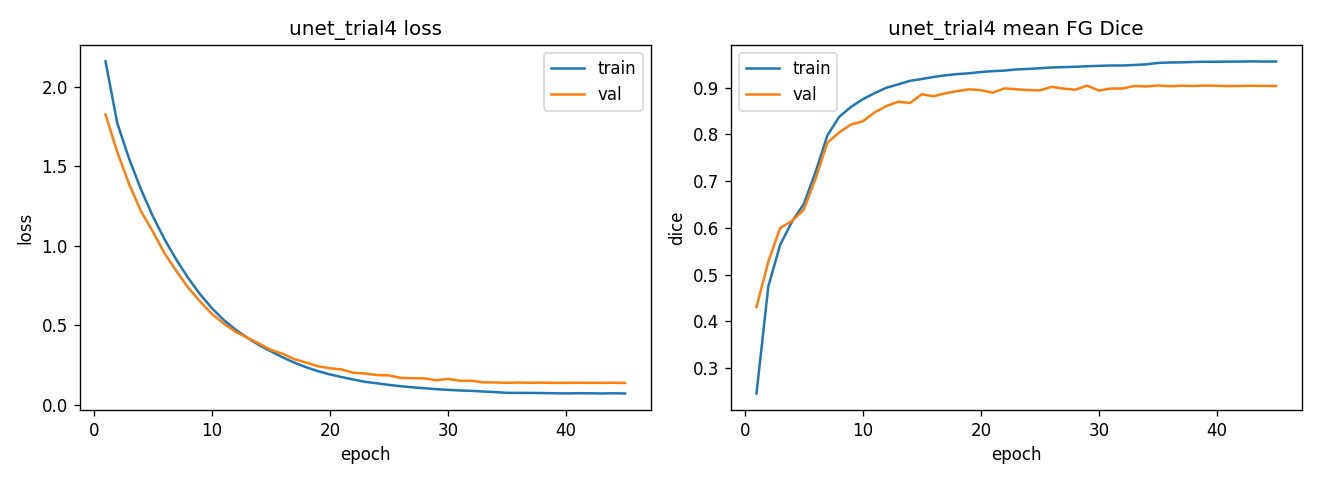
\includegraphics[width=\linewidth]{unet_trial4_curves.png}\caption{Trial 4}\end{subfigure}\hfill
\begin{subfigure}{0.32\textwidth}\mbox{}\end{subfigure}
\caption{U-Net per-trial training curves (Optuna).}
\label{fig:unet-trials}
\end{figure}

\begin{figure}[H]
\centering
\begin{subfigure}{0.32\textwidth}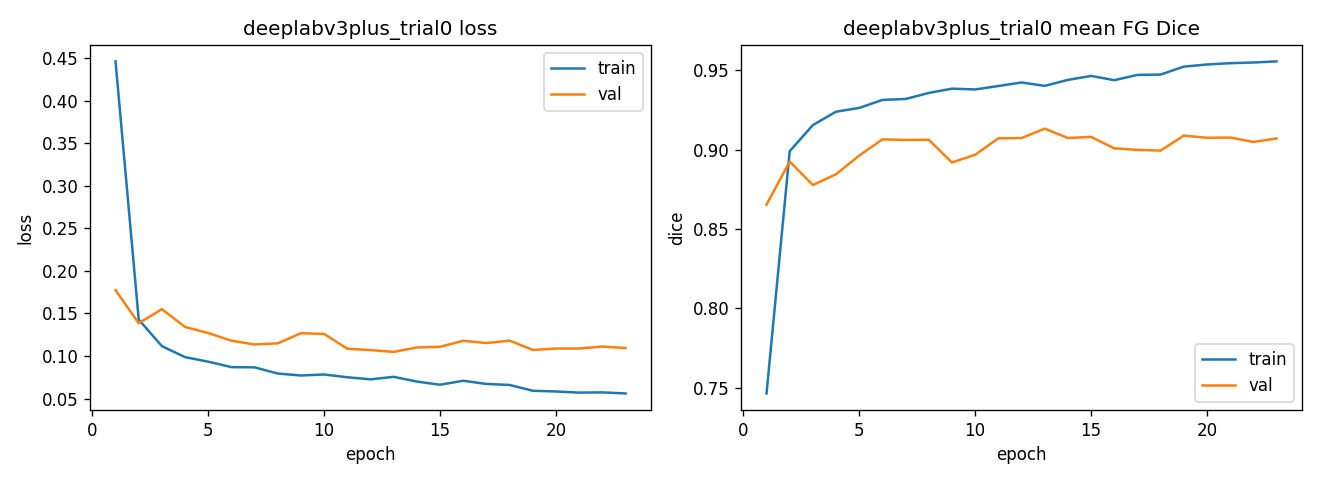
\includegraphics[width=\linewidth]{deeplabv3plus_trial0_curves.png}\caption{Trial 0 (best)}\end{subfigure}\hfill
\begin{subfigure}{0.32\textwidth}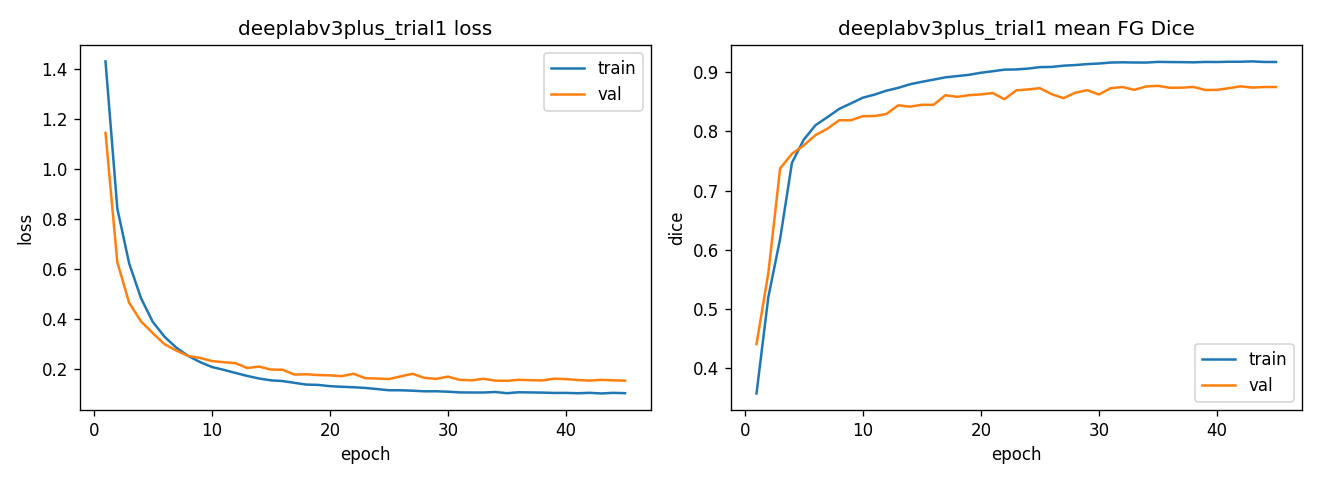
\includegraphics[width=\linewidth]{deeplabv3plus_trial1_curves.png}\caption{Trial 1}\end{subfigure}\hfill
\begin{subfigure}{0.32\textwidth}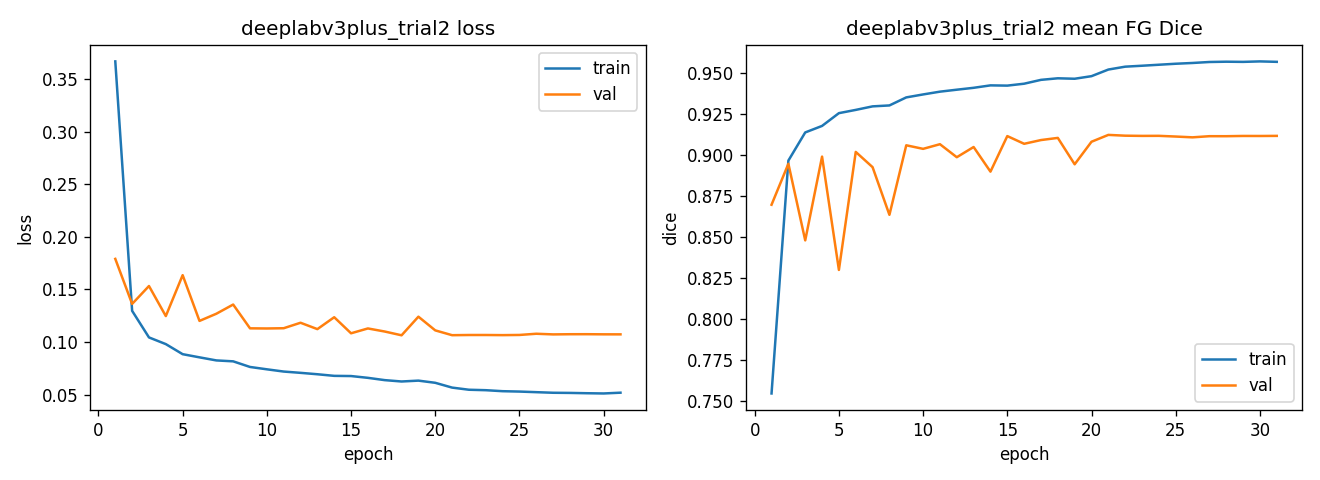
\includegraphics[width=\linewidth]{deeplabv3plus_trial2_curves.png}\caption{Trial 2}\end{subfigure}
\\[0.4em]
\begin{subfigure}{0.32\textwidth}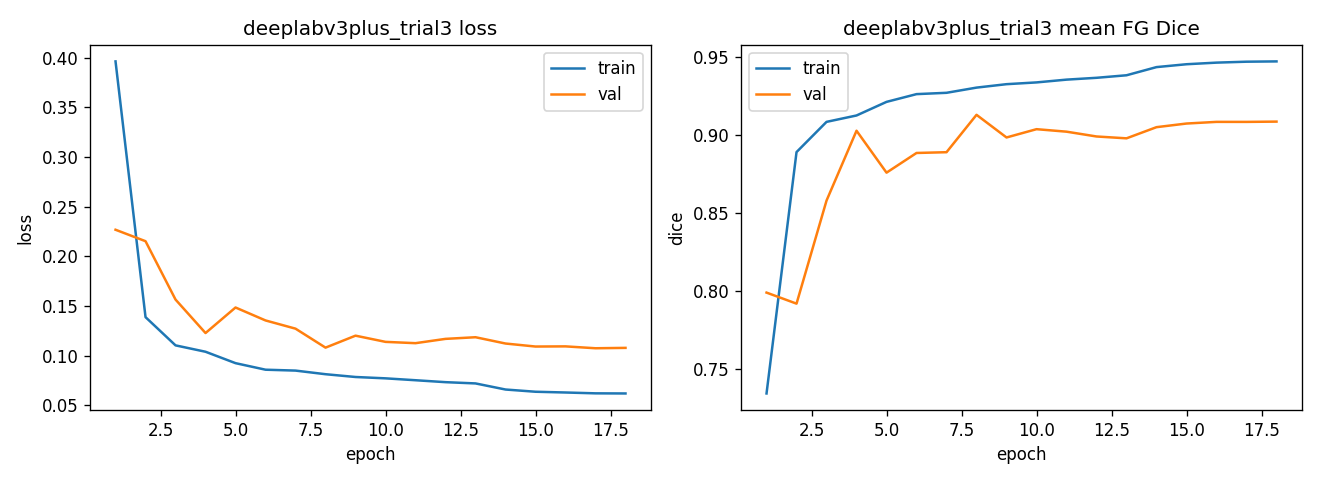
\includegraphics[width=\linewidth]{deeplabv3plus_trial3_curves.png}\caption{Trial 3}\end{subfigure}\hfill
\begin{subfigure}{0.32\textwidth}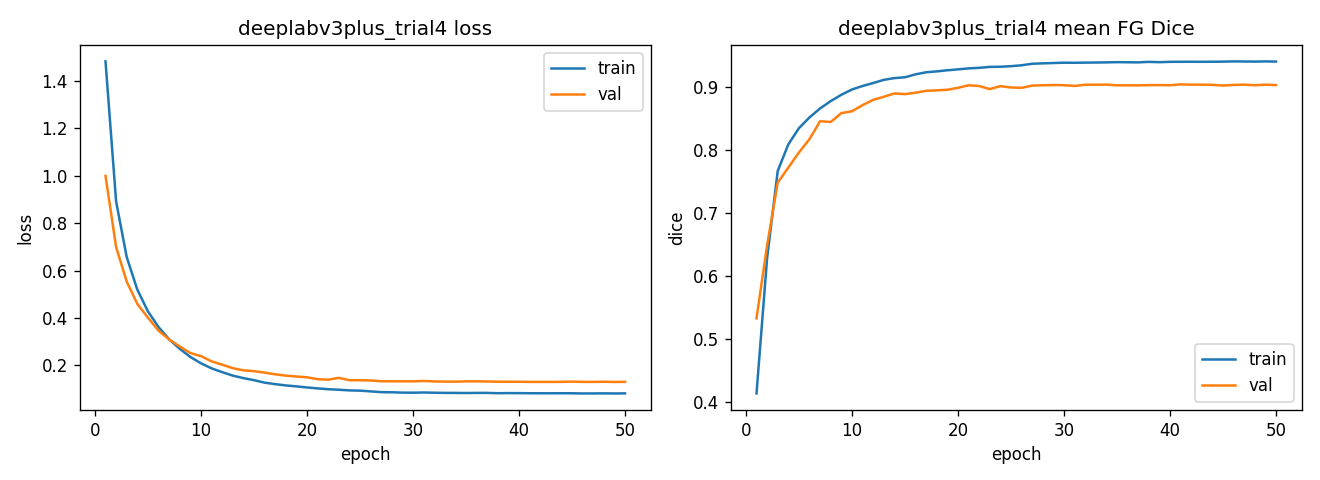
\includegraphics[width=\linewidth]{deeplabv3plus_trial4_curves.png}\caption{Trial 4}\end{subfigure}\hfill
\begin{subfigure}{0.32\textwidth}\mbox{}\end{subfigure}
\caption{DeepLabV3+ per-trial training curves (Optuna).}
\label{fig:deeplab-trials}
\end{figure}

%==================================================================
\section{Conclusions and Limitations}
%==================================================================
\begin{itemize}
  \item \textbf{U-Net is the stronger model here}, primarily because it segments the small,
        scattered infection regions far better (Dice 0.79 vs.\ 0.64, sensitivity 0.77 vs.\ 0.50).
  \item \textbf{Lung segmentation is essentially solved} by both architectures
        (Dice $\approx$ 0.97--0.98) --- a large, high-contrast target.
  \item \textbf{Infection is the bottleneck}: tiny, low-contrast and heavily imbalanced.
        The Dice+CE loss and augmentation help but do not close the gap.
  \item \textbf{Small dataset (20 volumes).} Patient-level splitting keeps evaluation honest,
        but generalisation is limited; more volumes, 3D context, and lesion-focused losses are
        the natural next steps.
\end{itemize}

%==================================================================
\begin{thebibliography}{9}
\bibitem{ma2020} J.~Ma \emph{et al.}, ``Towards Data-Efficient Learning: A Benchmark for
  COVID-19 CT Lung and Infection Segmentation,'' Zenodo 3757476, 2020.
  \url{https://zenodo.org/records/3757476}. Licence: CC BY-NC-SA.
\bibitem{unet} O.~Ronneberger, P.~Fischer, T.~Brox, ``U-Net: Convolutional Networks for
  Biomedical Image Segmentation,'' MICCAI, 2015.
\bibitem{deeplab} L.-C.~Chen \emph{et al.}, ``Encoder--Decoder with Atrous Separable
  Convolution for Semantic Image Segmentation (DeepLabV3+),'' ECCV, 2018.
\bibitem{optuna} T.~Akiba \emph{et al.}, ``Optuna: A Next-generation Hyperparameter
  Optimization Framework,'' KDD, 2019.
\bibitem{smp} P.~Iakubovskii, ``Segmentation Models PyTorch,''
  \url{https://github.com/qubvel/segmentation_models.pytorch}, 2019.
\end{thebibliography}

\end{document}
